\documentclass[25pt, a0paper, portrait]{tikzposter}

\usepackage{blindtext}
\usepackage{comment}
\usepackage{authblk}
\geometry{paperwidth=36in,paperheight=36in}
\usetheme{Simple}
\title{\parbox{\linewidth}{\centering Protein Complex Prediction Through Ensemble Clustering and Dynamic PPI Networks}}
% \author{Ali Hamza, Usaid Rehman, Haris K. Ladhani, Maham S. Patel, Dr. Humaira Jamshed}
% \title{some random bullsshit}
\author[1]{Ali Hamza}
\author[1]{M. Usaid Rehman}
\author[1]{Haris K. Ladhani}
\author[1]{Maham S. Patel}
\author[2]{Humaira Jamshed}
\date{\today}
\institute{Habib University}
\affil[1]{Dhanani School of Science \& Engineering, Habib University}
\affil[2]{Integrated Sciences \& Mathematics, Habib University} 

\makeatletter
\def\maketitle{\AB@maketitle}
\makeatother

\begin{document}
\maketitle
\block{~}
{
   {\large Protein-Protein Interaction (PPI) is an upcoming field with limitless 
potential which can help us understanding viral receptor binding and 
aid drug development among other things. Both in-vitro and in-vivo 
methods have limitations which is why in-silico methods are gaining 
popularity among proteomics researchers. However, the current method 
often falls short offering a room for innovation. Our aim is to create 
a PPI prediction algorithm that accounts for the topological and 
biological information whilst making its prediction. Our PPI prediction algorithm will create a more comprehensive and accurate database. We 
will be using generative models to account for accurate limited data 
that is currently available, and static and dynamic PPI networks to 
account for a more realistic PPI representation. We will, thereby, 
create a prediction algorithm using ensemble clustering methods to 
better predict PPI using topological and biological information present in the PPI networks.} \\

\textbf{Keywords:} Protein-Protein Interaction Networks, Ensemble Clustering, Prediction Model, PPI Database 
}

\begin{columns}
    \column{0.5}
    \block[ bodyoffsety=2cm,
  titleoffsety=2cm]{Background}
    {
        Protein-protein interactions are an important area of study in proteomics. When a large amount of proteins interact, they form protein-protein interaction (PPI) networks. These networks are widely studied in bioinformatics because they lend themselves to computational techniques quite naturally. 
        PPI networks can be modelled as combinatorial graphs and therefore, graph theoretical methods and algorithms can be applied to them. 
        
        Protein complexes are groups of proteins that interact together and display certain properties. Protein complexes form subgraphs in a PPI network. Identifying protein complexes 
        is a major problem in PPI network analysis where clustering methods can be used to detect complexes in PPI networks. We attempt to use ensemble clustering along with preexisting clustering algorithms to find a more accurate method to predict protein complexes. 
    }
     \block[ bodyoffsety=2cm,
  titleoffsety=2cm]{Overview of Proposed Pipeline}
    {
        \begin{tikzfigure}
            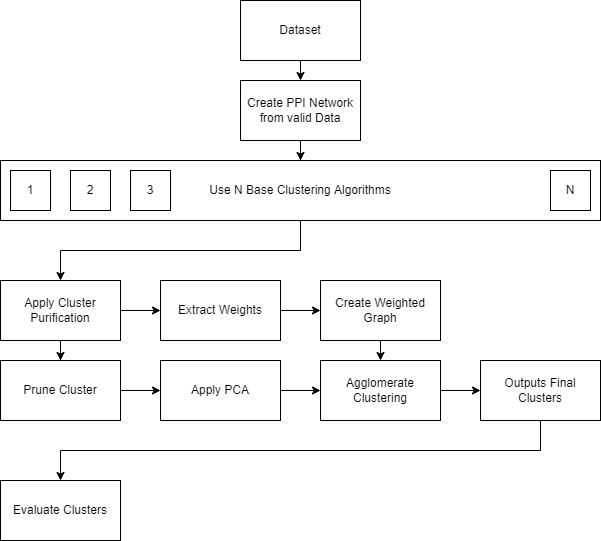
\includegraphics[width=0.35\textwidth]{images/systemdiag.png}
        \end{tikzfigure}
    }
    \column{0.5}
    \block[ bodyoffsety=2cm,
  titleoffsety=2cm]{Dataset}
    {
        PPI network datasets used for the purpose of this research have been extracted from primary sources such as BioGrid, MINT and Mentha as well as secondary or predictive databases such as String and primarily focus on a selected few species such as humans, mice, rats and yeast. The extraction process works by first collecting all possible proteins and their gene names for our selected species and then running queries for the extraction of PPI datasets for the respective proteins on online repositories. The datasets are then stored in a seperate database which contains a list of proteins and their interactions.
    }
 
    \block[bodyoffsety=2cm, titleoffsety=2cm]
    {Methodology}{
       Ensemble clustering is a promising method for protein complex identification problem. It relies on the use of $N$ number of base clustering algorithms which output a set of clusters for each algorithm.
       These different sets of clusters then go through the cluster purification stage where inconsistent clusters are discarded. Then dimensionality reduction is done through principal component analysis (PCA) in order to proceed to the final stage which is consensus clustering where the final clusters are obtained. 
       Our proposed method incorporates both biological and topological information in order to achieve more accurate results and to expand the list of features upon which complex prediction takes place. An overview of our pipeline can be seen on the left.
    }
    
    
    
    \block[ bodyoffsety=2cm,
  titleoffsety=2cm]{Results}{
    The results obtained by a lot of preexisting methods/algorithms are quite promising; however, they have certain limitations.
    Most methods do not account for sparse protein complexes, while some are fairly restrictive in their initial assumptions about topological properties of the complexes and do not incorporate any biological data. Our proposed method promises to improve upon these limitations and will be able to create a more accurate method that can improve current protein complex datasets.
  }
  
  
  \block[ bodyoffsety=2cm,
  titleoffsety=2cm]{Conclusion}{
    Our work can provide a better, more accurate and consistent protein complex identification method.
    Our proposed method for protein complex identification can help improve our understanding of how diseases progress and this would also help in drug development. 
  }

\end{columns}
\end{document}
